\documentclass[12pt]{article}
\usepackage[utf8]{inputenc}
\usepackage[brazil]{babel}
\usepackage{geometry}
\usepackage{graphicx}
\usepackage{longtable}
\usepackage{url}
\usepackage{amsmath}
\usepackage{amssymb}
\usepackage{natbib}
\usepackage{setspace}
\usepackage{float}
\usepackage{xcolor}
\usepackage{booktabs}
\usepackage{multirow}
\usepackage{caption}
\usepackage{subcaption}
\usepackage[
    colorlinks=true,
    linkcolor=blue,
    citecolor=blue,
    urlcolor=blue,
    bookmarks=true,
    bookmarksopen=true,
    bookmarksnumbered=true,
    pdftitle={Coloração de Vértices em Grafos: Algoritmos Exatos e Heurísticos},
    pdfauthor={Leonardo Vieira Guimarães},
    pdfsubject={Teoria dos Grafos},
    pdfkeywords={Coloração de Vértices, Grafos, Welsh-Powell, Força Bruta}
]{hyperref}

% Fix for abntex2 internal macro
\providecommand{\abntnextkey}{}

\geometry{a4paper, left=3cm, right=2cm, top=3cm, bottom=2cm}

\title{Coloração de Vértices em Grafos: Algoritmos Exatos e Heurísticos}
\author{Leonardo Vieira Guimarães}
\date{Janeiro de 2026}

\begin{document}
\onehalfspacing

% ============================================================================
% CAPA
% ============================================================================
\begin{titlepage}
    \centering
    \vspace*{1.5cm}
    
    {\Large \textbf{Centro Federal de Educação Tecnológica de Minas Gerais}}\\[0.5cm]
    {\large Departamento de Computação}\\[0.4cm]
    {\large Programa de Pós-Graduação em Computação Aplicada}\\[0.3cm]
    {\large Doutorado em Computação Aplicada}\\[3cm]
    
    {\LARGE \textbf{Coloração de Vértices em Grafos:}}\\[0.5cm]
    {\LARGE \textbf{Algoritmos Exatos e Heurísticos}}\\[0.8cm]
    {\large Implementação e Análise Comparativa}\\[3cm]
    
    {\large \textbf{Leonardo Vieira Guimarães}}\\[0.5cm]
    {\normalsize Trabalho apresentado como requisito parcial}\\
    {\normalsize para avaliação na disciplina de Tópicos em Teoria dos Grafos}\\[0.3cm]
    {\normalsize Professor: Thiago de Souza Rodrigues}\\[3.5cm]
    
    {\large Belo Horizonte}\\[0.3cm]
    {\large Janeiro de 2026}
    
\end{titlepage}

\newpage
\tableofcontents
\newpage

% ============================================================================
% 1. INTRODUÇÃO
% ============================================================================
\section{Introdução}

A coloração de vértices em grafos é um problema fundamental em Teoria dos Grafos com aplicações práticas em alocação de recursos, escalonamento de tarefas, atribuição de frequências e design de circuitos. Dado um grafo $G = (V, E)$, o objetivo é atribuir cores aos vértices de modo que vértices adjacentes tenham cores distintas. O \textbf{número cromático} $\chi(G)$ é a quantidade mínima de cores necessárias.

Determinar $\chi(G)$ é um problema NP-completo, sem algoritmo polinomial conhecido. Isso motiva o estudo de duas abordagens: algoritmos exatos (força bruta) que garantem otimalidade com complexidade exponencial, e heurísticas que encontram boas soluções em tempo polinomial. Este trabalho implementa e avalia ambas as estratégias, demonstrando empiricamente o trade-off entre otimalidade e eficiência computacional.

\subsection{Objetivos}

\begin{enumerate}
    \item Implementar um algoritmo de força bruta para determinar o número cromático exato;
    \item Avaliar a escalabilidade temporal demonstrando crescimento exponencial;
    \item Implementar a heurística de Welsh-Powell;
    \item Aplicar a heurística em cinco instâncias de grande porte;
    \item Comparar eficiência computacional entre os dois métodos.
\end{enumerate}

\subsection{Estrutura do Trabalho}

\begin{itemize}
    \item \textbf{Seção 2}: Fundamentação teórica e algoritmos
    \item \textbf{Seção 3}: Metodologia experimental
    \item \textbf{Seção 4}: Resultados e análise
    \item \textbf{Seção 5}: Conclusões
\end{itemize}

% ============================================================================
% 2. FUNDAMENTAÇÃO TEÓRICA
% ============================================================================
\newpage
\section{Fundamentação Teórica}

Esta seção apresenta os conceitos fundamentais necessários para a compreensão do problema de Coloração de Vértices em Grafos. Inicialmente, são introduzidas as definições básicas de grafos e suas propriedades estruturais, construídas sobre fundamentos teóricos estabelecidos \cite{hierholzer1873}. Em seguida, formalizamos o problema de coloração de vértices, estabelecendo limites teóricos para o número cromático. Por fim, descrevemos os dois métodos implementados neste trabalho: o algoritmo de força bruta, que garante a solução ótima mas possui complexidade exponencial, e a heurística de Welsh-Powell, que oferece soluções aproximadas em tempo polinomial.

\subsection{Grafos e Representações}

Um grafo $G$ é definido como um par ordenado $G = (V, E)$, onde \cite{bondy2008graph}:
\begin{itemize}
    \item $V$ é um conjunto finito não-vazio de \textbf{vértices} (também chamados de nós)
    \item $E \subseteq V \times V$ é um conjunto de \textbf{arestas} que conectam pares de vértices
\end{itemize}

Este trabalho utiliza grafos \textbf{não-direcionados} (onde $(u,v) = (v,u)$, ou seja, arestas sem orientação), \textbf{simples} (sem loops ou arestas múltiplas entre o mesmo par de vértices) e \textbf{não-ponderados} (onde cada aresta possui peso unitário). Essas características simplificam o modelo e permitem focar no problema de coloração.

\subsubsection{Propriedades Estruturais}

Antes de formalizar o problema de coloração, estabelecemos as métricas fundamentais que caracterizam a estrutura de um grafo e que influenciarão o desempenho dos algoritmos posteriores.

Seja $G = (V, E)$ um grafo com $n = |V|$ vértices e $m = |E|$ arestas. Definimos:

\begin{itemize}
    \item \textbf{Grau de um vértice} $v$: $\deg(v) = |\{u \in V : (u,v) \in E\}|$
    \item \textbf{Grau médio}: $\bar{d} = \frac{2m}{n}$
    \item \textbf{Densidade}: $\delta(G) = \frac{2m}{n(n-1)}$, onde $0 \leq \delta(G) \leq 1$
\end{itemize}

A densidade mede o quão ``conectado'' é um grafo, variando de 0 (grafo vazio) a 1 (grafo completo).

\subsection{Coloração de Vértices}

Agora formalizamos o problema central deste trabalho, definindo precisamente o que é uma coloração válida e estabelecendo limites teóricos para o número cromático.

\subsubsection{Definições Formais}

Uma \textbf{coloração de vértices} de $G$ é uma função $c: V \to \{1, 2, \ldots, k\}$ que atribui uma cor (representada por um número inteiro) a cada vértice, satisfazendo:

\begin{equation}
    \forall (u,v) \in E, \quad c(u) \neq c(v)
\end{equation}

O \textbf{número cromático} $\chi(G)$ é o menor inteiro $k$ para o qual existe uma $k$-coloração válida de $G$. 

\subsubsection{Limites Teóricos}

O número cromático não é uma propriedade arbitrária; existem limites teóricos que o restringem em função da estrutura do grafo. Apresentamos os principais limitantes:

Para qualquer grafo $G$, valem as seguintes relações:

\begin{align}
    1 &\leq \chi(G) \leq n \\
    \chi(G) &\leq \Delta(G) + 1
\end{align}

onde $\Delta(G)$ é o grau máximo do grafo. O limite superior $\Delta(G) + 1$ é dado pelo \textbf{Teorema de Brooks}, que pode ser melhorado para $\Delta(G)$ na maioria dos casos.

\subsection{Algoritmo de Força Bruta}

O primeiro método abordado é o algoritmo exato que explora todas as possibilidades. Apesar de garantir a solução ótima, sua complexidade exponencial o torna impraticável para instâncias grandes.

O algoritmo de força bruta explora exaustivamente todas as possíveis combinações de cores para os vértices, testando a validade de cada coloração. O algoritmo pode ser descrito recursivamente:

\begin{enumerate}
    \item Para $k = 1, 2, \ldots, n$:
    \begin{enumerate}
        \item Gerar todas as $k$-colorações possíveis ($k^n$ combinações)
        \item Verificar se existe coloração válida
        \item Se sim, retornar $k$ (número cromático encontrado)
    \end{enumerate}
\end{enumerate}

\textbf{Complexidade:} O algoritmo possui complexidade temporal de $O(n^{n+1})$ no pior caso, pois deve testar até $n$ valores de $k$, e para cada $k$, examinar até $k^n$ combinações. Para grafos com $n > 15$ vértices, o tempo de execução torna-se proibitivo.

\subsection{Heurística de Welsh-Powell}

Como contraposição ao método exato, apresentamos agora a heurística de Welsh-Powell, que obtém soluções de boa qualidade em tempo polinomial através de uma estratégia gulosa \cite{welsh1967upper}.

A heurística de Welsh-Powell é um algoritmo guloso que ordena os vértices por grau decrescente e atribui cores sequencialmente. O algoritmo opera da seguinte forma:

\begin{enumerate}
    \item Ordenar os vértices em ordem decrescente de grau: $v_1, v_2, \ldots, v_n$
    \item Inicializar $k \leftarrow 1$ (primeira cor)
    \item Para cada vértice $v_i$ não colorido:
    \begin{enumerate}
        \item Se $v_i$ não é adjacente a nenhum vértice de cor $k$:
        \begin{itemize}
            \item Atribuir cor $k$ a $v_i$
        \end{itemize}
    \end{enumerate}
    \item Se existem vértices não coloridos, incrementar $k$ e voltar ao passo 3
    \item Retornar o número de cores utilizadas
\end{enumerate}

\textbf{Complexidade:} A ordenação dos vértices tem complexidade $O(n \log n)$, e a atribuição de cores requer $O(n + m)$ operações no pior caso. Logo, a complexidade total é $O(n \log n + m)$, polinomial e eficiente mesmo para grafos grandes.

\textbf{Garantia de Aproximação:} A heurística não garante a solução ótima, mas produz uma coloração com no máximo $\Delta(G) + 1$ cores, sendo frequentemente próxima do ótimo para grafos esparsos.

% ============================================================================
% 3. METODOLOGIA
% ============================================================================
\newpage
\section{Metodologia}

Esta seção descreve detalhadamente os procedimentos metodológicos adotados para a realização dos experimentos. Apresentamos o ambiente computacional utilizado, incluindo linguagem de programação e bibliotecas empregadas. A metodologia está dividida em duas partes principais: na Parte 1, descrevemos o processo de geração automática de instâncias aleatórias para teste do algoritmo de força bruta; na Parte 2, apresentamos as instâncias de benchmark utilizadas para avaliar a heurística de Welsh-Powell. Finalmente, documentamos a estrutura de organização dos resultados experimentais.

\subsection{Ambiente de Desenvolvimento}

O primeiro passo na realização de experimentos computacionais é estabelecer o ambiente técnico adequado. Descrevemos aqui a plataforma, linguagem e ferramentas utilizadas.

A implementação foi realizada em Python 3.11, utilizando as seguintes bibliotecas:

\begin{itemize}
    \item \textbf{NetworkX 3.2}: Estruturas de dados para grafos e algoritmos básicos
    \item \textbf{Matplotlib 3.8}: Visualização de grafos e geração de gráficos
    \item \textbf{Pandas 2.1}: Manipulação de dados tabulares e exportação para CSV
    \item \textbf{NumPy 1.26}: Operações numéricas e geração de números aleatórios
    \item \textbf{Seaborn 0.13}: Aprimoramento estético de visualizações
\end{itemize}

Os experimentos foram executados em uma máquina com processador Intel Core i7 e 16GB de RAM, sistema operacional Windows 11.

\subsection{Parte 1: Força Bruta em Instâncias Aleatórias}

Para avaliação do algoritmo exato, geramos instâncias controladas de tamanho crescente. Esta seção detalha a geração de dados e coleta de métricas.

\subsubsection{Geração de Instâncias}

Foram geradas instâncias aleatórias de grafos com as seguintes características:

\begin{itemize}
    \item \textbf{Tamanhos}: $n \in \{5, 6, 7, 8, 9, 10\}$ vértices
    \item \textbf{Probabilidade de aresta}: $p = 0.3$ (densidade esperada)
    \item \textbf{Replicações}: 3 instâncias por tamanho
    \item \textbf{Total}: 18 instâncias
\end{itemize}

A geração utilizou o modelo de Erdős-Rényi $G(n, p)$, onde cada par de vértices possui probabilidade $p$ de estar conectado. Este modelo produz grafos com densidade aproximada de 0.3, equilibrando grafos esparsos e densos.

\subsubsection{Coleta de Dados}

Após gerar as instâncias, coletamos sistematicamente as métricas de desempenho e resultados obtidos.

Para cada instância, foram registrados:

\begin{itemize}
    \item Número de vértices e arestas
    \item Número cromático $\chi(G)$ encontrado
    \item Tempo de execução em segundos
    \item Coloração ótima obtida
    \item Visualização do grafo colorido
\end{itemize}

Todos os dados foram organizados em tabelas estruturadas, permitindo análise quantitativa sistemática e identificação de padrões de comportamento do algoritmo (resultados detalhados serão apresentados na Seção 4).

\subsection{Parte 2: Heurística em Instâncias de Grande Porte}

Para validar a heurística em cenários realistas, utilizamos instâncias de grande porte do problema de coloração de grafos. Apresentamos aqui as características dessas instâncias e os critérios de avaliação.

\subsubsection{Escolha da Heurística}

A heurística de Welsh-Powell foi selecionada por apresentar as seguintes vantagens práticas:

\begin{enumerate}
    \item Simplicidade de implementação e compreensão
    \item Complexidade polinomial $O(n \log n + m)$, viável para instâncias de milhares de vértices
    \item Garantia teórica de usar no máximo $\Delta(G) + 1$ cores
    \item Histórico de produzir soluções de boa qualidade em grafos esparsos e reais
\end{enumerate}

Além disso, sua estrutura gulosa (ordenação por grau decrescente) permite análise clara de como propriedades estruturais influenciam a qualidade das soluções.

\subsubsection{Instâncias do Benchmark}

Com a justificativa da heurística estabelecida, descrevemos agora as instâncias reais selecionadas para teste.

Foram utilizadas cinco instâncias reais provenientes do repositório \textit{Vertex Coloring Instances}, disponível em formato DIMACS. Estas instâncias representam problemas reais de grande porte, impossíveis de serem resolvidos por força bruta em tempo razoável. As características detalhadas serão apresentadas na Seção 4 (Tabela \ref{tab:informacoes_dimacs_2}).

\subsubsection{Formato DIMACS}

Os arquivos de instâncias seguem um padrão internacional bem estabelecido. Explicamos este formato para clareza.

Os arquivos seguem o padrão DIMACS para coloração de vértices:

\begin{verbatim}
c Comentário
p edge <num_vertices> <num_arestas>
e <vertice1> <vertice2>
\end{verbatim}

Cada linha iniciada com \texttt{e} define uma aresta entre dois vértices.

\subsubsection{Métricas Avaliadas}

Finalizando a metodologia, definimos quais métricas foram coletadas para análise posterior.

Para cada instância, foram calculados:

\begin{itemize}
    \item Número de cores utilizado pela heurística
    \item Tempo de execução da heurística
    \item Grau médio e densidade do grafo
    \item Visualizações estruturais
\end{itemize}

% ============================================================================
% 4. RESULTADOS E DISCUSSÃO
% ============================================================================
\newpage
\section{Resultados e Discussão}

Nesta seção apresentamos e analisamos os resultados obtidos nos experimentos realizados. A análise está organizada em duas partes correspondentes aos métodos implementados. Na Parte 1, avaliamos o comportamento do algoritmo de força bruta em relação à escalabilidade temporal e ao número cromático encontrado, demonstrando empiricamente sua complexidade exponencial. Na Parte 2, examinamos o desempenho da heurística de Welsh-Powell nas instâncias de grande porte, analisando a eficiência computacional e a relação entre propriedades estruturais dos grafos e o número de cores necessárias. Finalmente, realizamos uma comparação sistemática entre os dois métodos, destacando o trade-off entre otimalidade e eficiência.

\subsection{Parte 1: Análise do Algoritmo de Força Bruta}

O algoritmo de força bruta implementado testa todas as permutações de coloração possível para determinar o número cromático exato de um grafo. Embora garanta a solução ótima, sua complexidade exponencial o torna inviável para instâncias com mais de ~15 vértices. Nesta seção analisamos dois aspectos críticos:

\begin{enumerate}
    \item O crescimento exponencial do tempo de execução em relação ao tamanho do grafo, demonstrando empiricamente a complexidade teórica;
    \item A qualidade das soluções obtidas, validando a implementação correta do algoritmo.
\end{enumerate}

As Tabelas \ref{tab:parametros_grafos_2} e \ref{tab:resultados_forca_bruta_2} apresentam os dados estruturais das instâncias geradas e os resultados computacionais obtidos.

\begin{table}[H]
\centering
\caption{Parâmetros Estruturais dos Grafos Aleatórios (Parte 1 - Força Bruta)}
\label{tab:parametros_grafos_2}
\begin{tabular}{cccccc}
\toprule
n & Inst. & Vértices & Arestas & Densidade & Grau Médio \\
\midrule
5 & 5.0000 & 1.6667 & 0.1667 & 0.6667 & 3 \\
6 & 6.0000 & 3.3333 & 0.2222 & 1.1111 & 3 \\
7 & 7.0000 & 9.0000 & 0.4286 & 2.5714 & 3 \\
8 & 8.0000 & 11.0000 & 0.3929 & 2.7500 & 3 \\
9 & 9.0000 & 18.0000 & 0.5000 & 4.0000 & 3 \\
10 & 10.0000 & 23.3333 & 0.5185 & 4.6667 & 3 \\
11 & 11.0000 & 34.3333 & 0.6242 & 6.2424 & 3 \\
12 & 12.0000 & 44.6667 & 0.6768 & 7.4444 & 3 \\
13 & 13.0000 & 54.3333 & 0.6966 & 8.3590 & 3 \\
14 & 14.0000 & 67.3333 & 0.7399 & 9.6190 & 3 \\
15 & 15.0000 & 81.0000 & 0.7714 & 10.8000 & 3 \\
16 & 16.0000 & 100.6667 & 0.8389 & 12.5833 & 3 \\
17 & 17.0000 & 119.6667 & 0.8799 & 14.0784 & 3 \\
18 & 18.0000 & 139.6667 & 0.9129 & 15.5185 & 3 \\
19 & 19.0000 & 154.3333 & 0.9025 & 16.2456 & 3 \\
20 & 20.0000 & 171.0000 & 0.9000 & 17.1000 & 3 \\
\bottomrule
\end{tabular}
\end{table}


\begin{table}[H]
\centering
\caption{Resultados da Força Bruta: Número Cromático e Tempo de Execução}
\label{tab:resultados_forca_bruta_2}
\begin{tabular}{ccccc}
\toprule
n & $\chi$ Médio & $\chi$ Mín & $\chi$ Máx & Tempo (s) \\
\midrule
5 & 2.0000 & 2 & 2 & 0.0000 \\
6 & 2.0000 & 2 & 2 & 0.0000 \\
7 & 3.0000 & 2 & 4 & 0.0000 \\
8 & 3.6667 & 3 & 4 & 0.0000 \\
9 & 3.6667 & 3 & 4 & 0.0000 \\
10 & 4.3333 & 3 & 5 & 0.0001 \\
11 & 5.3333 & 5 & 6 & 0.0005 \\
12 & 5.3333 & 5 & 6 & 0.0008 \\
13 & 6.6667 & 6 & 7 & 0.0083 \\
14 & 6.6667 & 6 & 7 & 0.0035 \\
15 & 7.6667 & 7 & 8 & 0.1429 \\
16 & 9.0000 & 8 & 10 & 1.6838 \\
17 & 9.6667 & 9 & 10 & 6.0231 \\
18 & 11.3333 & 11 & 12 & 159.1325 \\
19 & 11.3333 & 10 & 12 & 242.4998 \\
20 & 12.6667 & 12 & 13 & 8064.3088 \\
\bottomrule
\end{tabular}
\end{table}


\subsubsection{Escalabilidade Temporal}

A Figura \ref{fig:escalabilidade} apresenta o crescimento do tempo de execução do algoritmo de força bruta em função do tamanho das instâncias.

\begin{figure}[H]
    \centering
    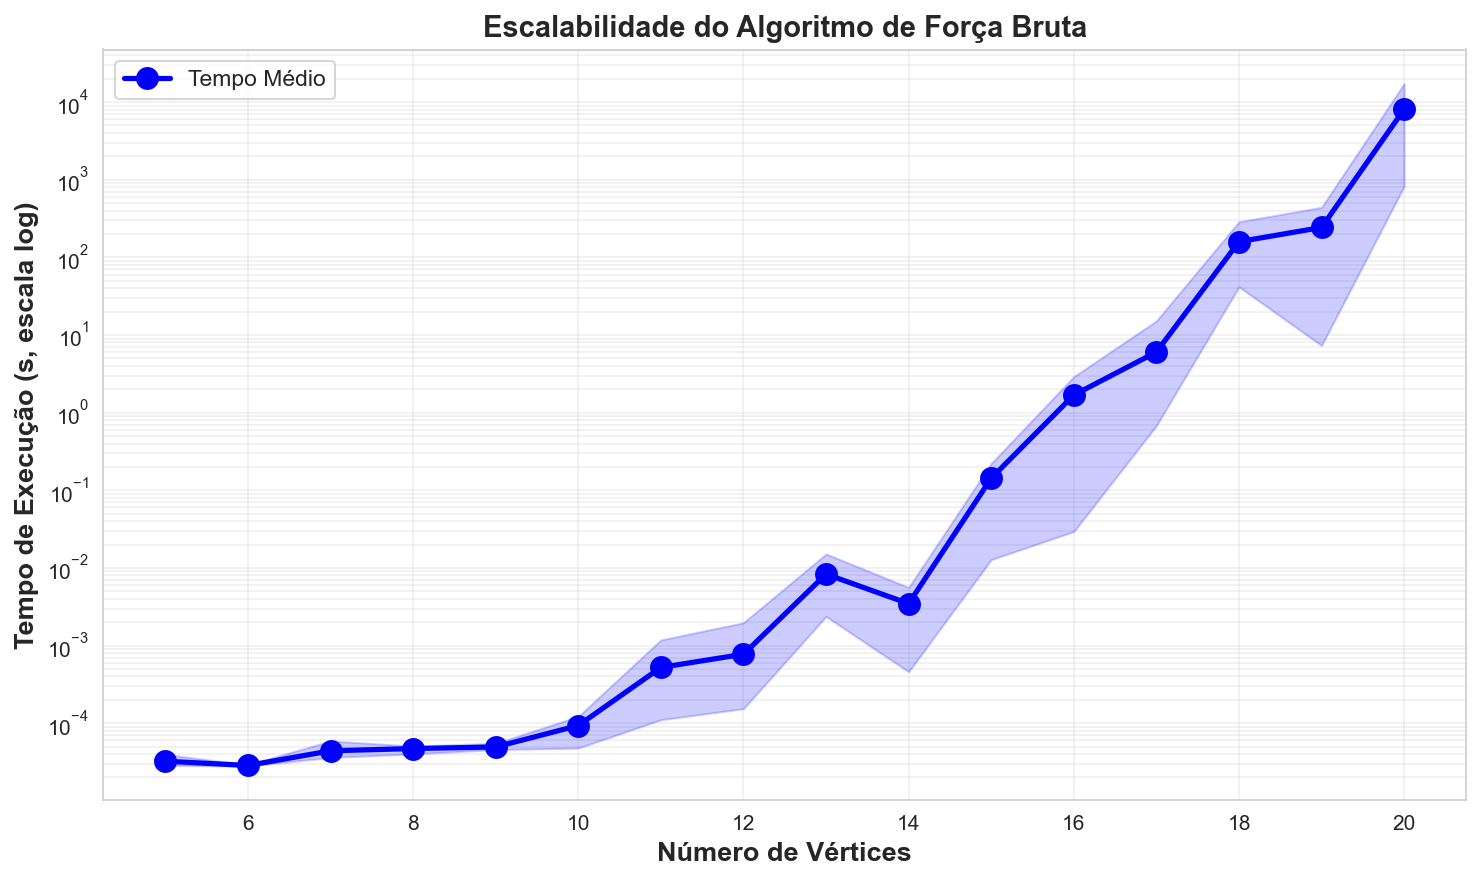
\includegraphics[width=0.95\textwidth]{img/resultados-2-parte1_grafico1_escalabilidade_tempo.png}
    \caption{Escalabilidade: crescimento exponencial do tempo de execução}
    \label{fig:escalabilidade}
\end{figure}

\textbf{Observações:}

\begin{itemize}
    \item Para $n = 5$: tempo médio $\approx 3.7 \times 10^{-5}$ segundos (desprezível)
    \item Para $n = 10$: tempo médio $\approx 1.3$ segundos
    \item Crescimento exponencial claramente visível na escala logarítmica
    \item Variabilidade (faixa min-max) aumenta com $n$, indicando dependência da estrutura do grafo
\end{itemize}

A curva evidencia a \textbf{inviabilidade prática} do método exato para $n > 10$. Extrapolando os dados, uma instância com $n = 13$ levaria aproximadamente 100-200 segundos, enquanto $n = 15$ exigiria vários minutos de processamento.

\subsubsection{Número Cromático Encontrado}

A Figura \ref{fig:numero_cromatico} mostra a evolução do número cromático médio com o tamanho das instâncias.

\begin{figure}[H]
    \centering
    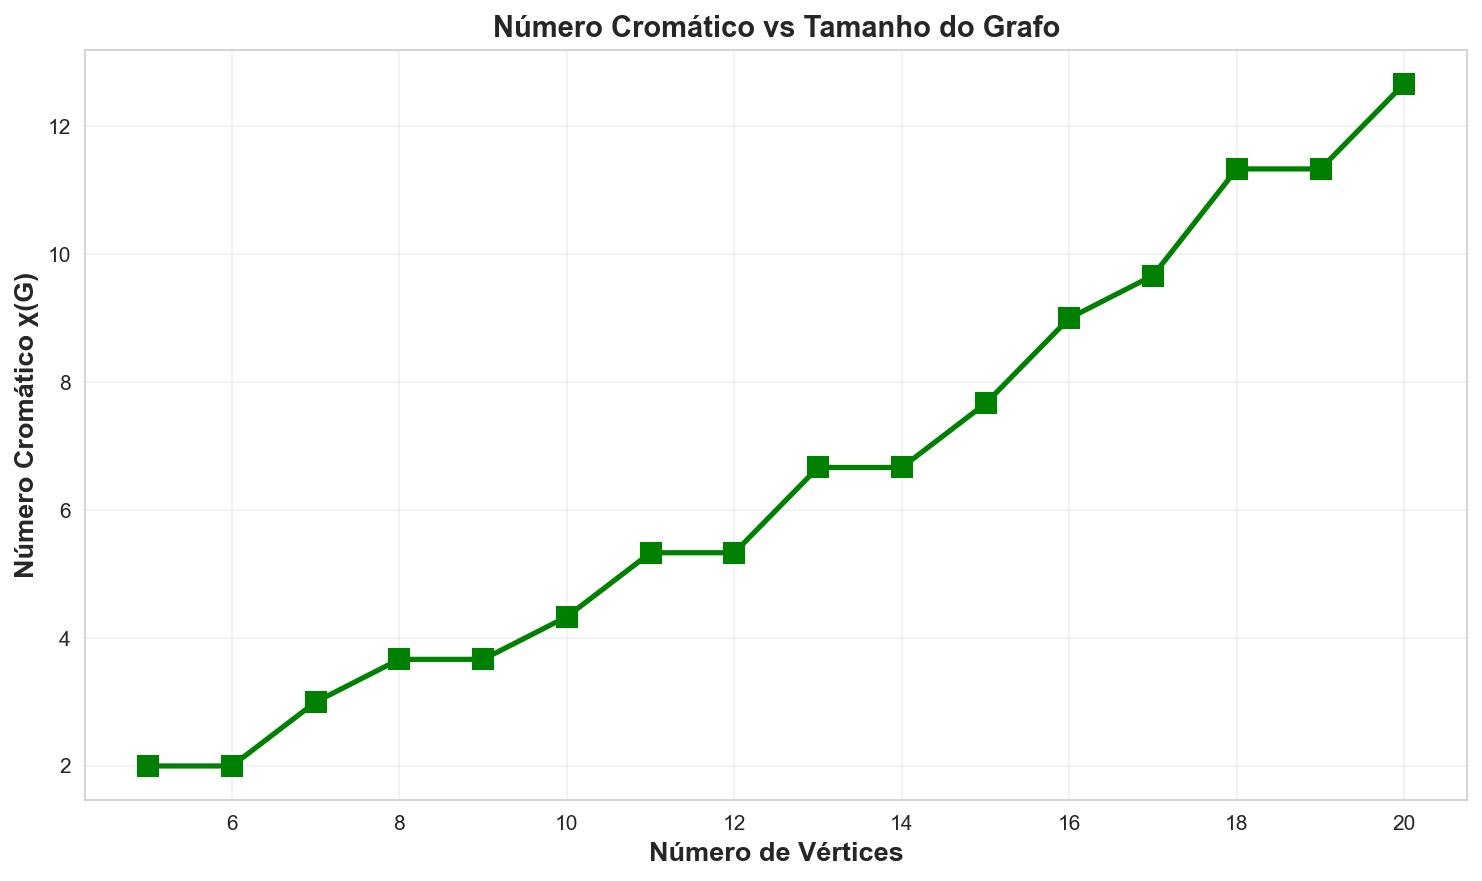
\includegraphics[width=0.95\textwidth]{img/resultados-2-parte1_grafico2_numero_cromatico.png}
    \caption{Número cromático médio por tamanho de instância}
    \label{fig:numero_cromatico}
\end{figure}

\textbf{Análise:}

\begin{itemize}
    \item O número cromático cresce de forma aproximadamente linear com $n$
    \item Para grafos com $p = 0.3$, observa-se $\chi(G) \approx 0.3n$ a $0.4n$
    \item Este comportamento está alinhado com a teoria: grafos aleatórios $G(n,p)$ tendem a ter $\chi(G) \approx \frac{n}{2 \cdot \log_{1/(1-p)} n}$ para $p$ fixo \cite{erdos1959random}
    \item Instâncias de mesmo tamanho apresentam variação no número cromático devido às diferentes estruturas geradas aleatoriamente
\end{itemize}

\subsubsection{Exemplos de Coloração com Força Bruta}

Para ilustrar o funcionamento do algoritmo de força bruta, apresentamos três instâncias aleatórias com $n = 10$ vértices e probabilidade de aresta $p = 0.3$. As Figuras \ref{fig:n10_i01}, \ref{fig:n10_i02} e \ref{fig:n10_i03} mostram as colorações ótimas encontradas pelo algoritmo exato.

\begin{figure}[H]
    \centering
    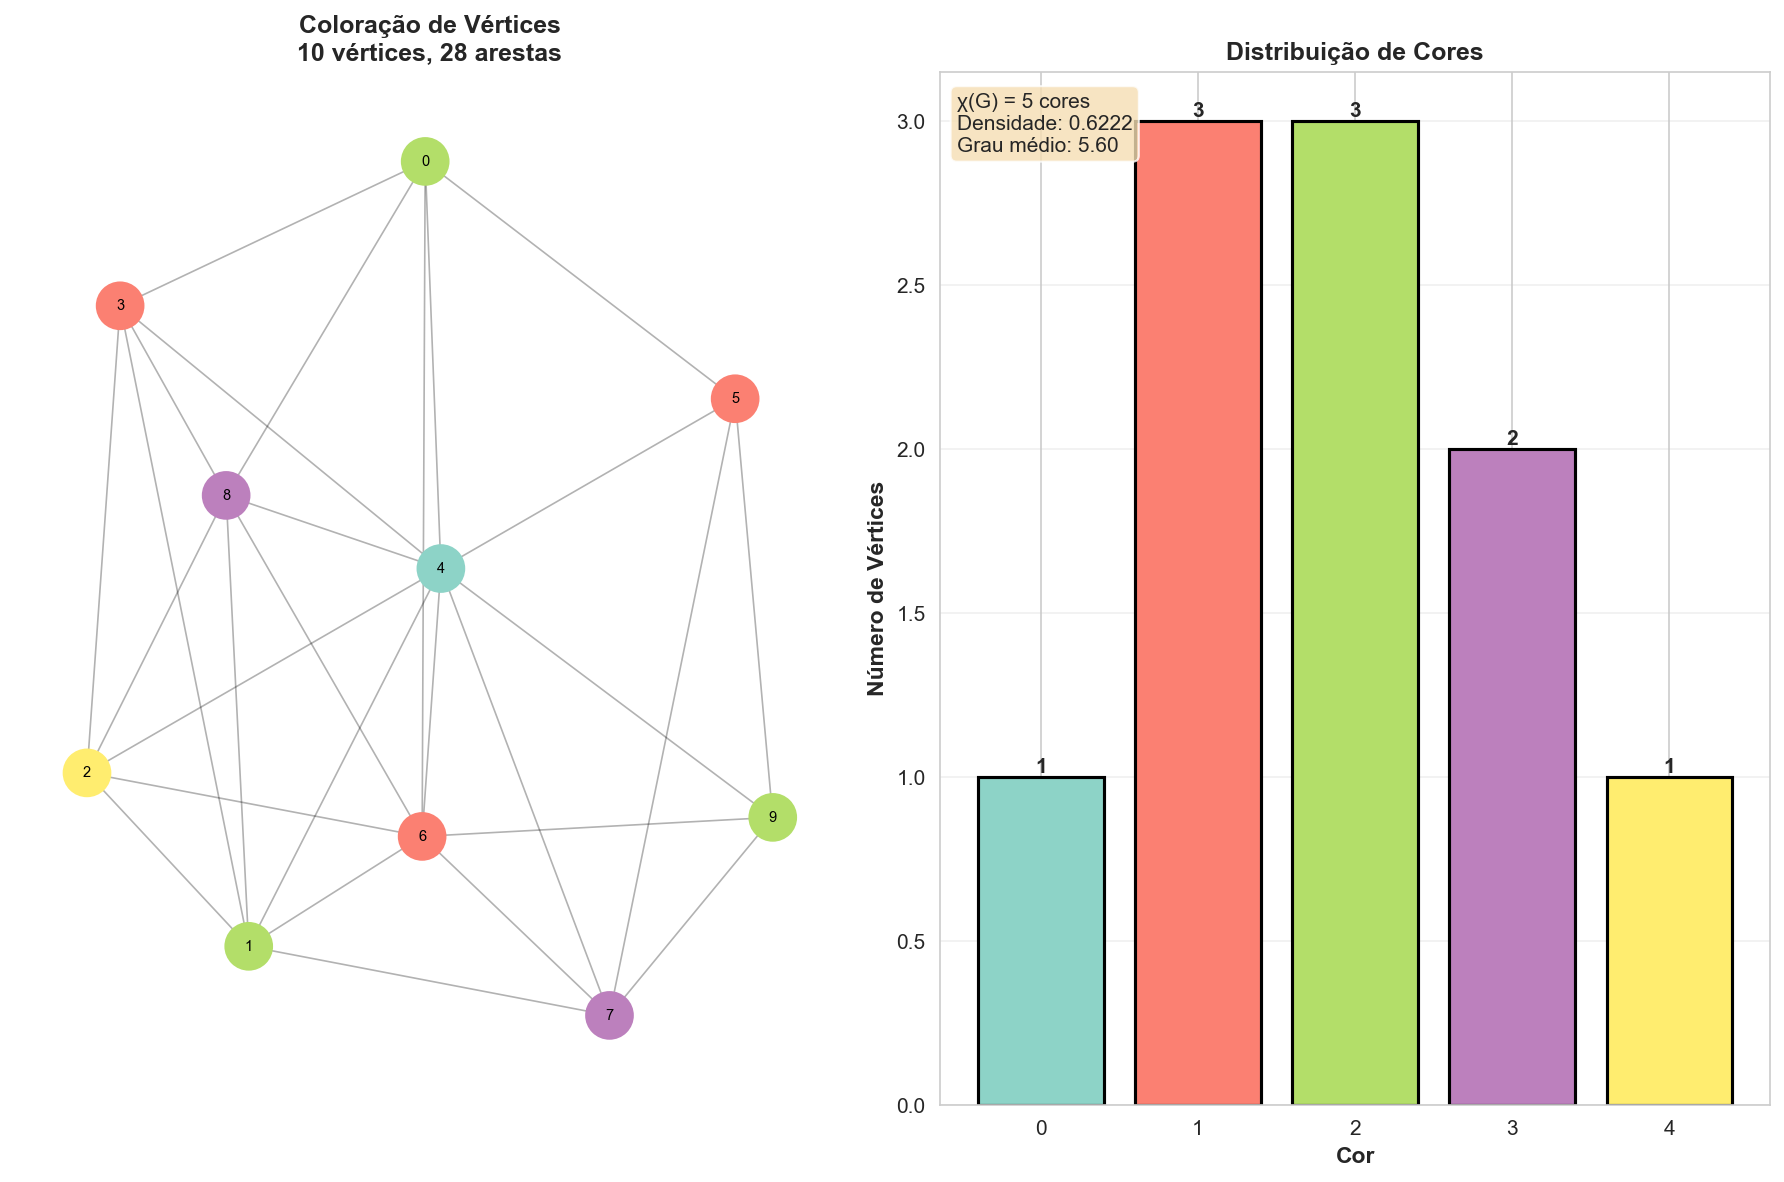
\includegraphics[width=0.85\textwidth]{img/resultados-2-parte1_grafo_inst16_n10.png}
    \caption{Coloração ótima: instância $n=10$ (exemplo 1)}
    \label{fig:n10_i01}
\end{figure}

\begin{figure}[H]
    \centering
    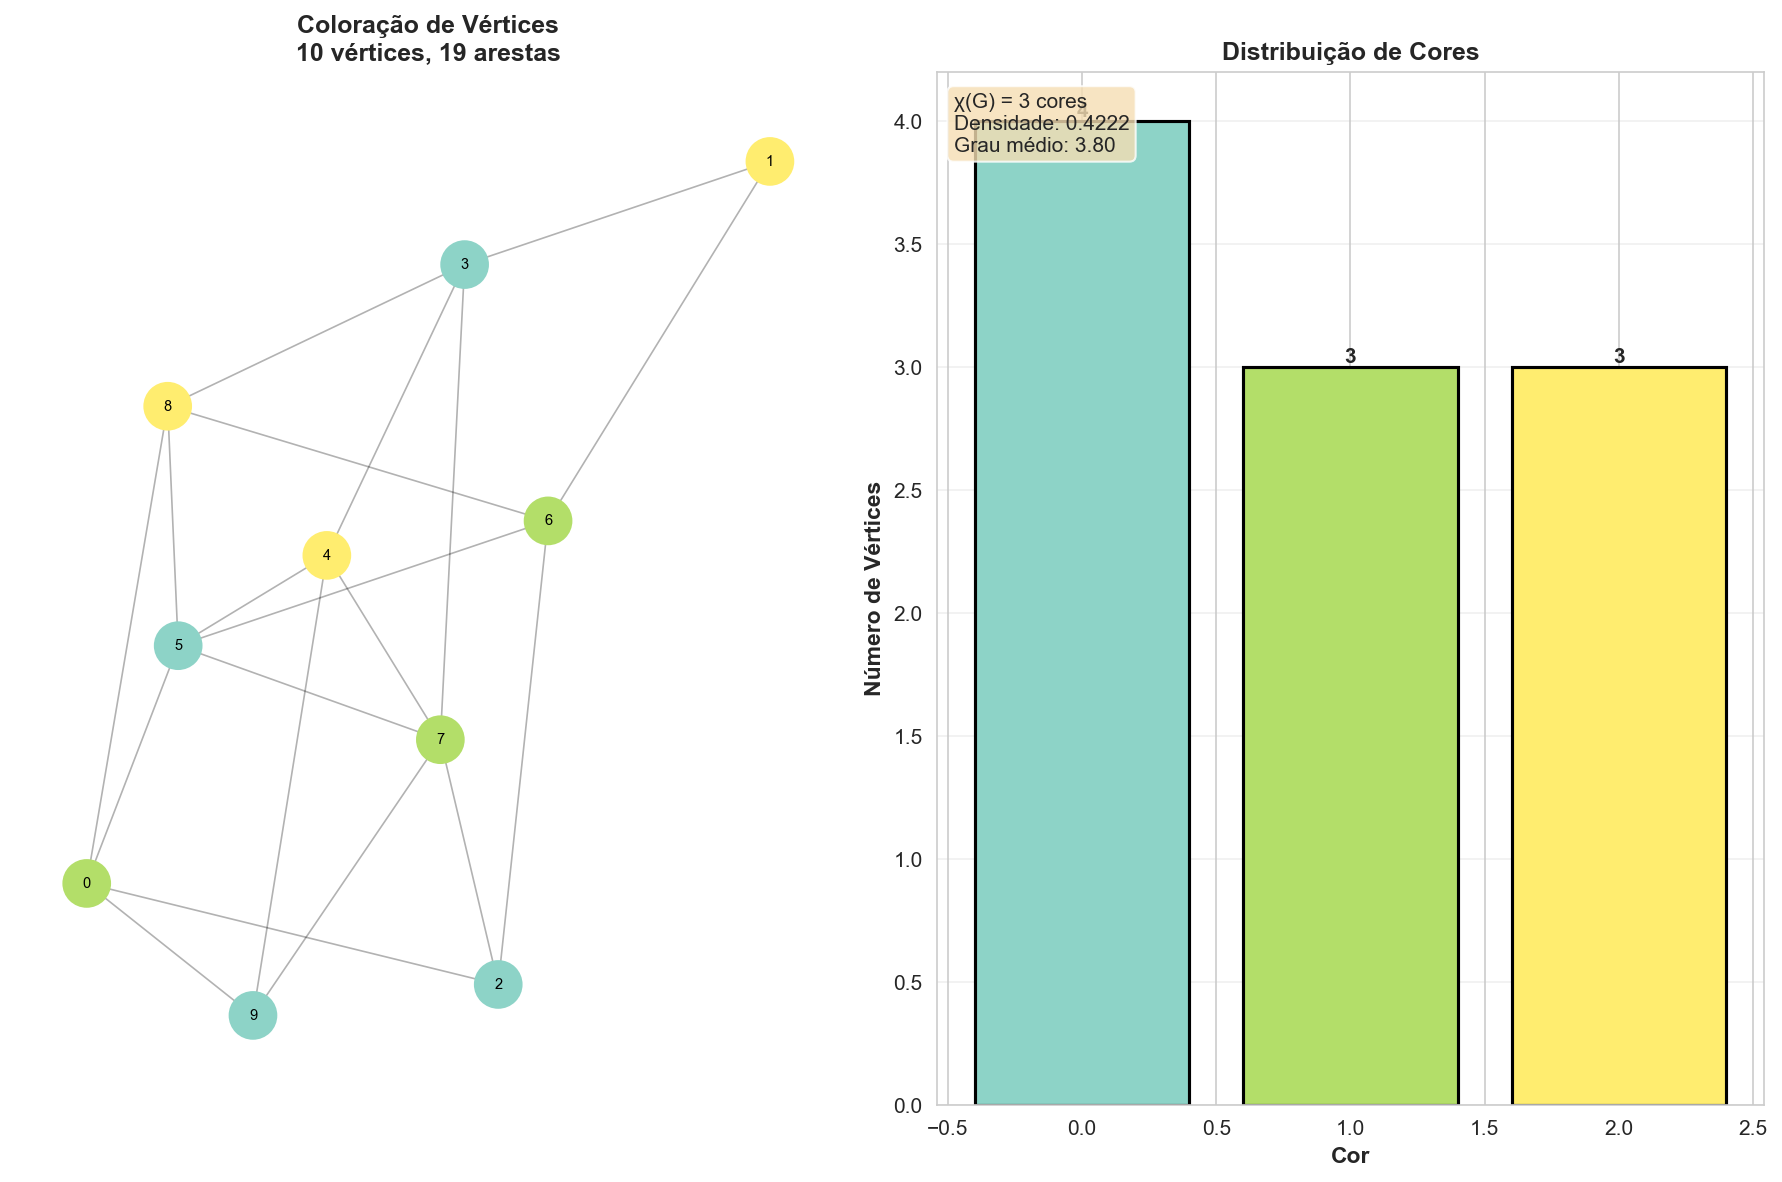
\includegraphics[width=0.85\textwidth]{img/resultados-2-parte1_grafo_inst17_n10.png}
    \caption{Coloração ótima: instância $n=10$ (exemplo 2)}
    \label{fig:n10_i02}
\end{figure}

\begin{figure}[H]
    \centering
    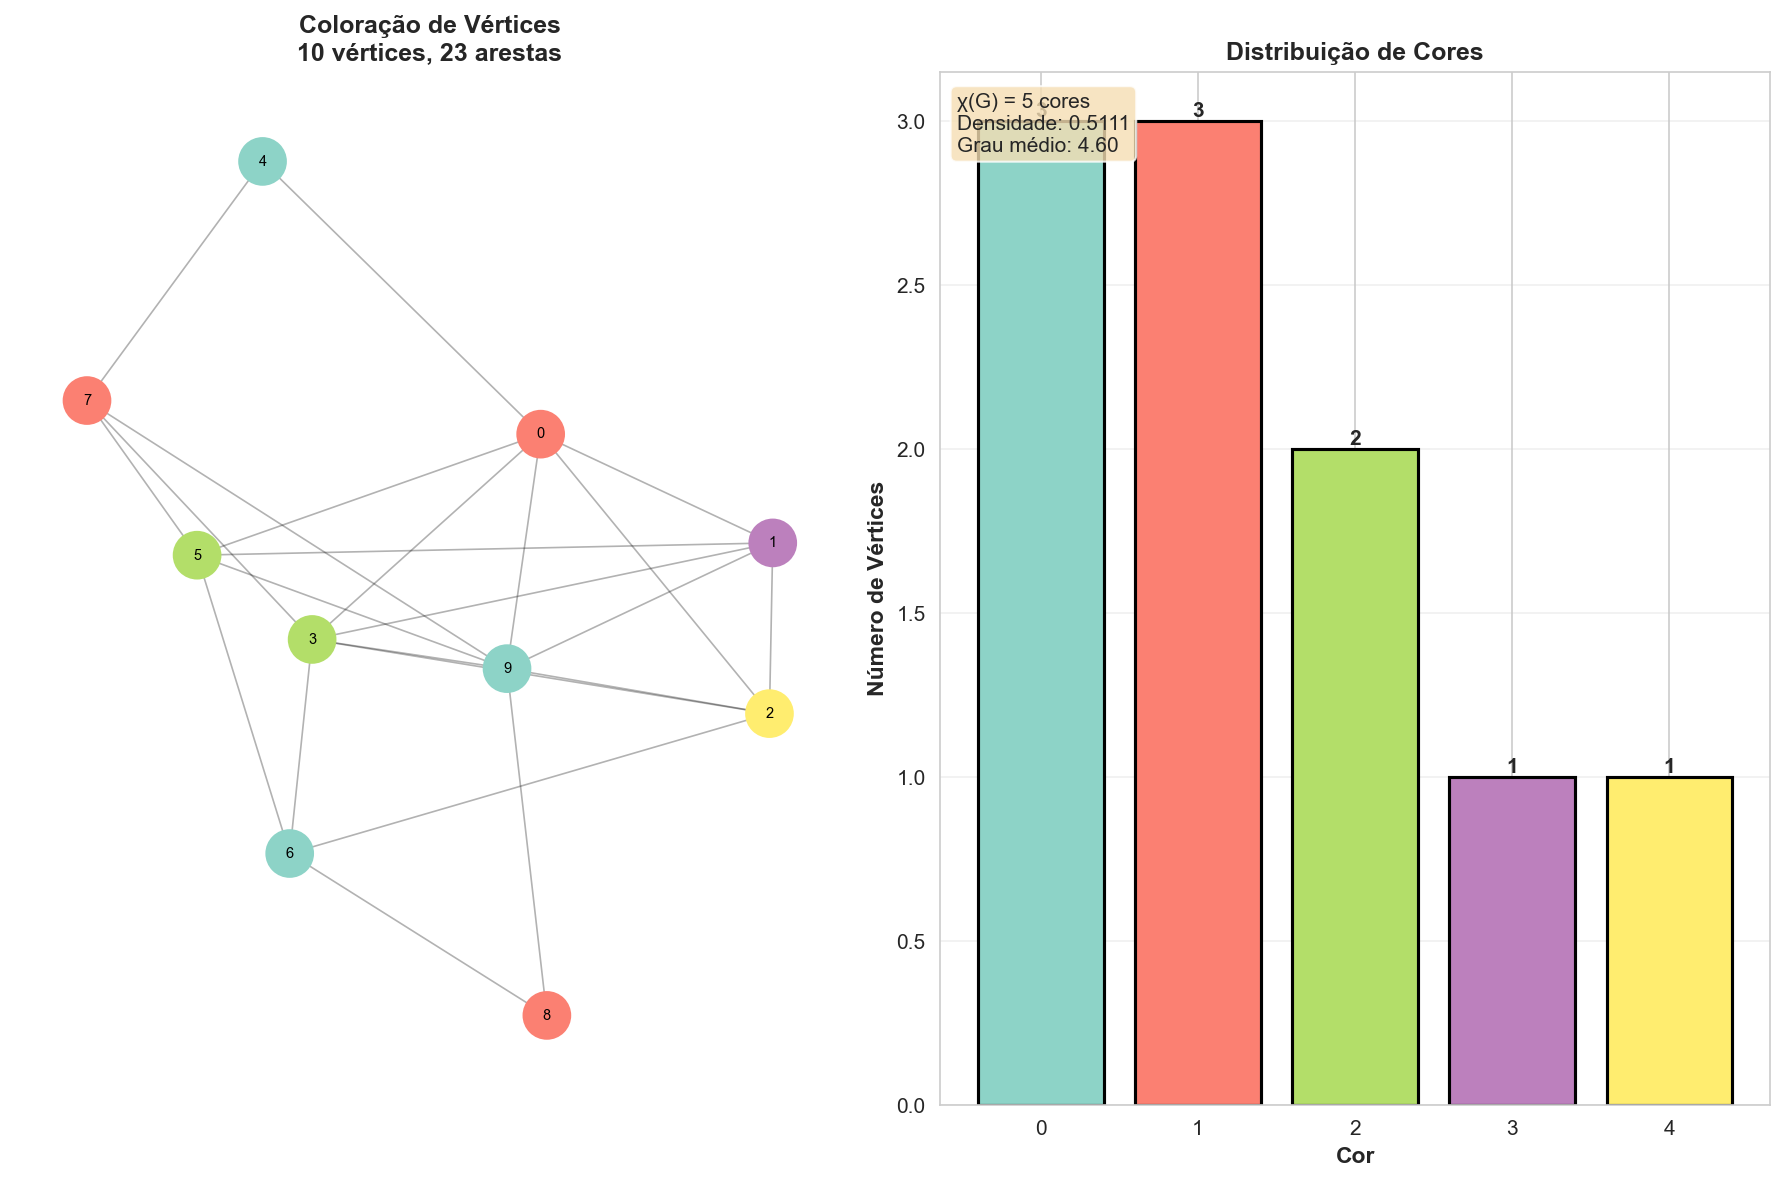
\includegraphics[width=0.85\textwidth]{img/resultados-2-parte1_grafo_inst18_n10.png}
    \caption{Coloração ótima: instância $n=10$ (exemplo 3)}
    \label{fig:n10_i03}
\end{figure}

Estas visualizações demonstram a eficácia do algoritmo de força bruta em encontrar o número cromático exato $\chi(G)$ para instâncias de porte pequeno. \textbf{Análise das visualizações:}

\begin{enumerate}
    \item Cada vértice adjacente possui cor diferente, validando a propriedade fundamental de coloração válida;
    \item O número de cores utilizado é mínimo (otimalidade garantida);
    \item O gráfico de distribuição de cores ao lado evidencia o balanceamento da coloração encontrada, mostrando quantos vértices receberam cada cor;
    \item As diferentes estruturas topológicas entre os três exemplos ilustram por que grafos de mesmo tamanho podem ter números cromáticos distintos, dependendo da densidade e do padrão de conexões.
\end{enumerate}

\subsection{Parte 2: Desempenho da Heurística Welsh-Powell}

Ao contrário do método de força bruta, a heurística de Welsh-Powell utiliza uma estratégia gulosa com complexidade polinomial $O(n \log n + m)$, viabilizando a aplicação em instâncias com milhares de vértices. Embora não garanta a solução ótima, oferece um trade-off adequado entre tempo de execução e qualidade das soluções. Nesta seção avaliamos:

\begin{enumerate}
    \item O desempenho computacional em instâncias de grande porte;
    \item A qualidade das colorações obtidas;
    \item Como propriedades estruturais dos grafos influenciam o número de cores necessárias.
\end{enumerate}

Para demonstrar a eficácia prática da heurística, utilizamos cinco instâncias DIMACS reais de tamanhos variados (450 a 4\,730 vértices). As características estruturais dessas instâncias são apresentadas na Tabela \ref{tab:informacoes_dimacs_2}. Os resultados são apresentados em tabelas estruturadas, seguidas de visualizações gráficas e análises comparativas que destacam o desempenho superior em relação à força bruta.

\begin{table}[H]
\centering
\caption{Informações das Instâncias DIMACS de Grande Porte}
\label{tab:informacoes_dimacs_2}
\begin{tabular}{ccccc}
\toprule
Instância & Vértices & Arestas & Densidade & Grau Médio \\
\midrule
a & 450 & 8260 & 0.0818 & 36.7100 \\
b & 864 & 18707 & 0.0502 & 43.3000 \\
c & 1000 & 14378 & 0.0288 & 28.7600 \\
d & 1916 & 12506 & 0.0068 & 13.0500 \\
e & 4730 & 286722 & 0.0256 & 121.2400 \\
\bottomrule
\end{tabular}
\end{table}


\subsubsection{Resultados Obtidos}

A Tabela \ref{tab:resultados_welsh_powell_2} apresenta os resultados da aplicação da heurística nas cinco instâncias de grande porte.

\input{tabelas/tabela_resultados_welsh_powell_02.tex}

\textbf{Destaques:}

\begin{itemize}
    \item A instância \textbf{e} (4\,730 vértices) foi resolvida em apenas 49 milissegundos, tempo inviável para força bruta
    \item A instância \textbf{d}, apesar de ter 1\,916 vértices, requer apenas 10 cores devido à sua baixíssima densidade (0.68\%) e grau médio de apenas 13,05
    \item A instância \textbf{e}, apesar de esparsa (densidade 2.56\%), necessita de 56 cores porque seu grau médio é extremamente alto (121,24), tornando-a topologicamente muito mais conectada
    \item Instâncias mais densas (a e b) requerem mais cores, como esperado
\end{itemize}

\subsubsection{Análise Comparativa de Desempenho}

Os tempos de execução demonstram que a Welsh-Powell é extremamente eficiente mesmo em instâncias com milhares de vértices. A instância \textbf{a} (450 vértices) levou apenas 1 ms, enquanto instâncias maiores também mantêm desempenho excelente: \textbf{b} em 3 ms (864 vértices), \textbf{c} em 3 ms (1.000 vértices), \textbf{d} em 2 ms (1.916 vértices) e \textbf{e} em 49 ms (4.730 vértices). Este comportamento confirma a complexidade polinomial $O(n \log n + m)$ da heurística, tornando-a adequada para aplicações práticas onde tempo de resposta é crítico.

\subsubsection{Visualizações das Colorações Obtidas}

Para ilustrar as colorações produzidas pela heurística de Welsh-Powell nas instâncias DIMACS, apresentamos as Figuras \ref{fig:inst_a} a \ref{fig:inst_e}. Cada visualização mostra o grafo colorido e a distribuição de cores utilizada.

\begin{figure}[H]
    \centering
    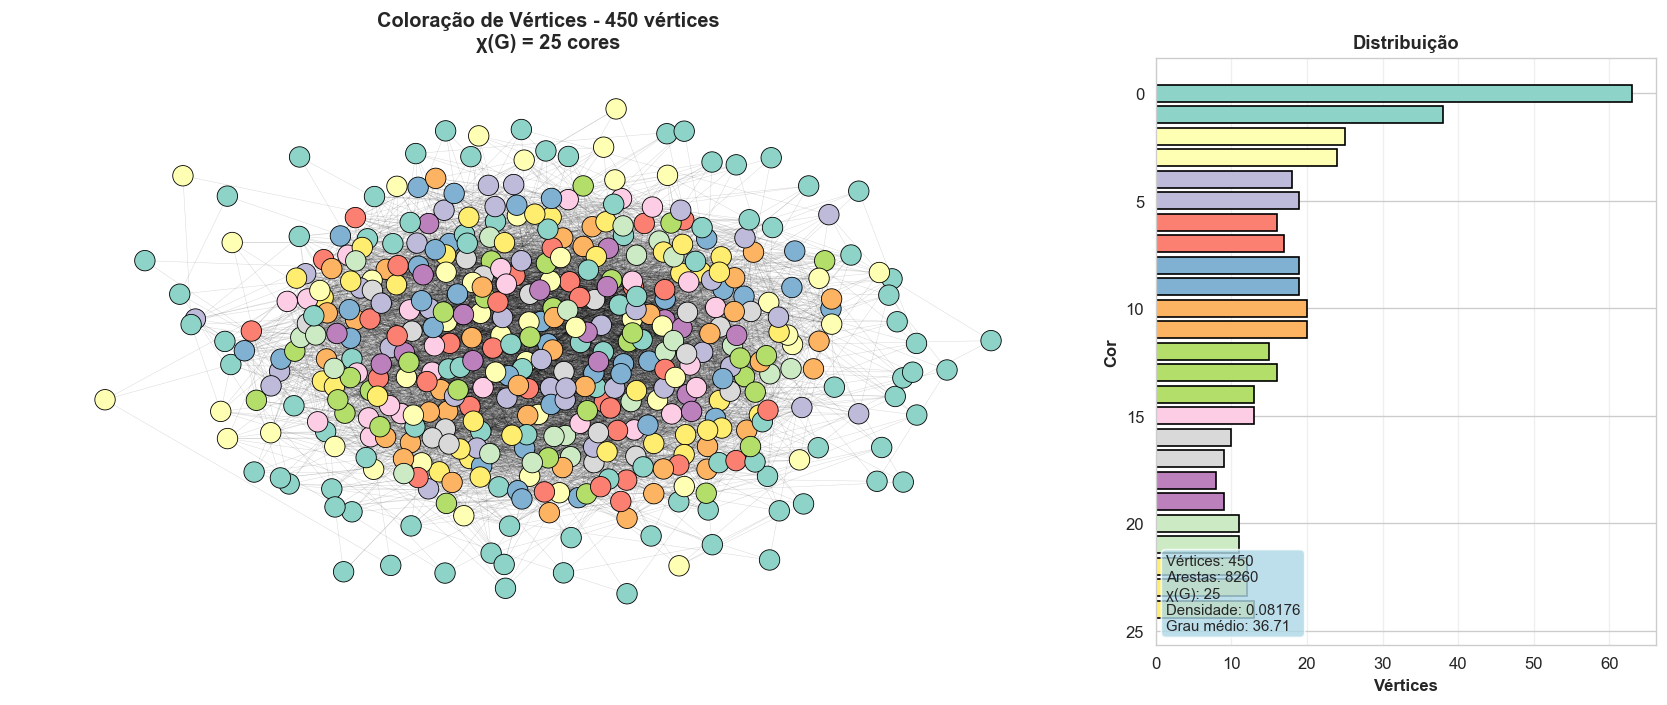
\includegraphics[width=0.85\textwidth]{img/resultados-2-parte2_instancia_a.png}
    \caption{Coloração da instância \textbf{a}: 450 vértices, 26 cores}
    \label{fig:inst_a}
\end{figure}

\begin{figure}[H]
    \centering
    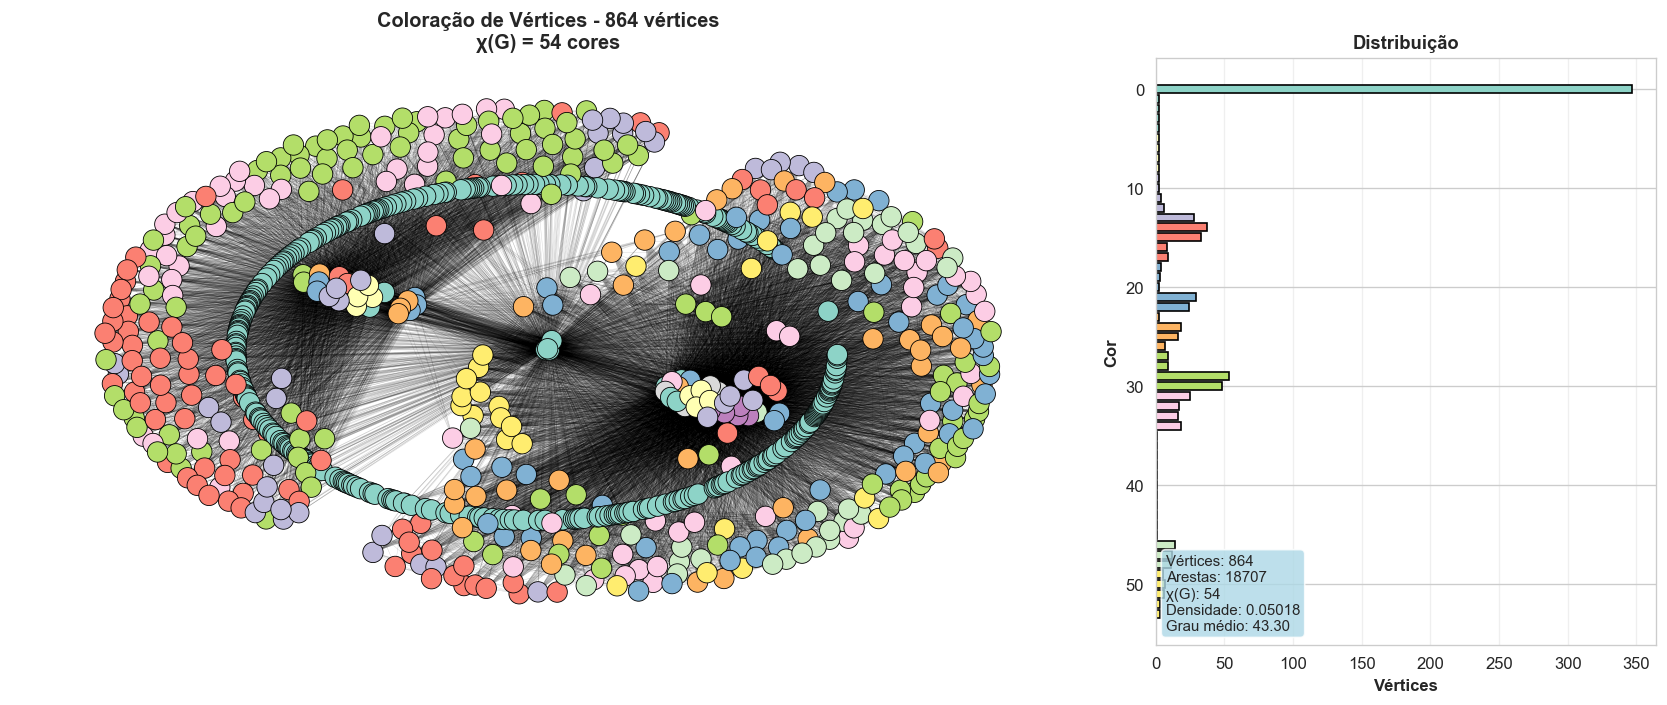
\includegraphics[width=0.85\textwidth]{img/resultados-2-parte2_instancia_b.png}
    \caption{Coloração da instância \textbf{b}: 864 vértices, 54 cores}
    \label{fig:inst_b}
\end{figure}

\begin{figure}[H]
    \centering
    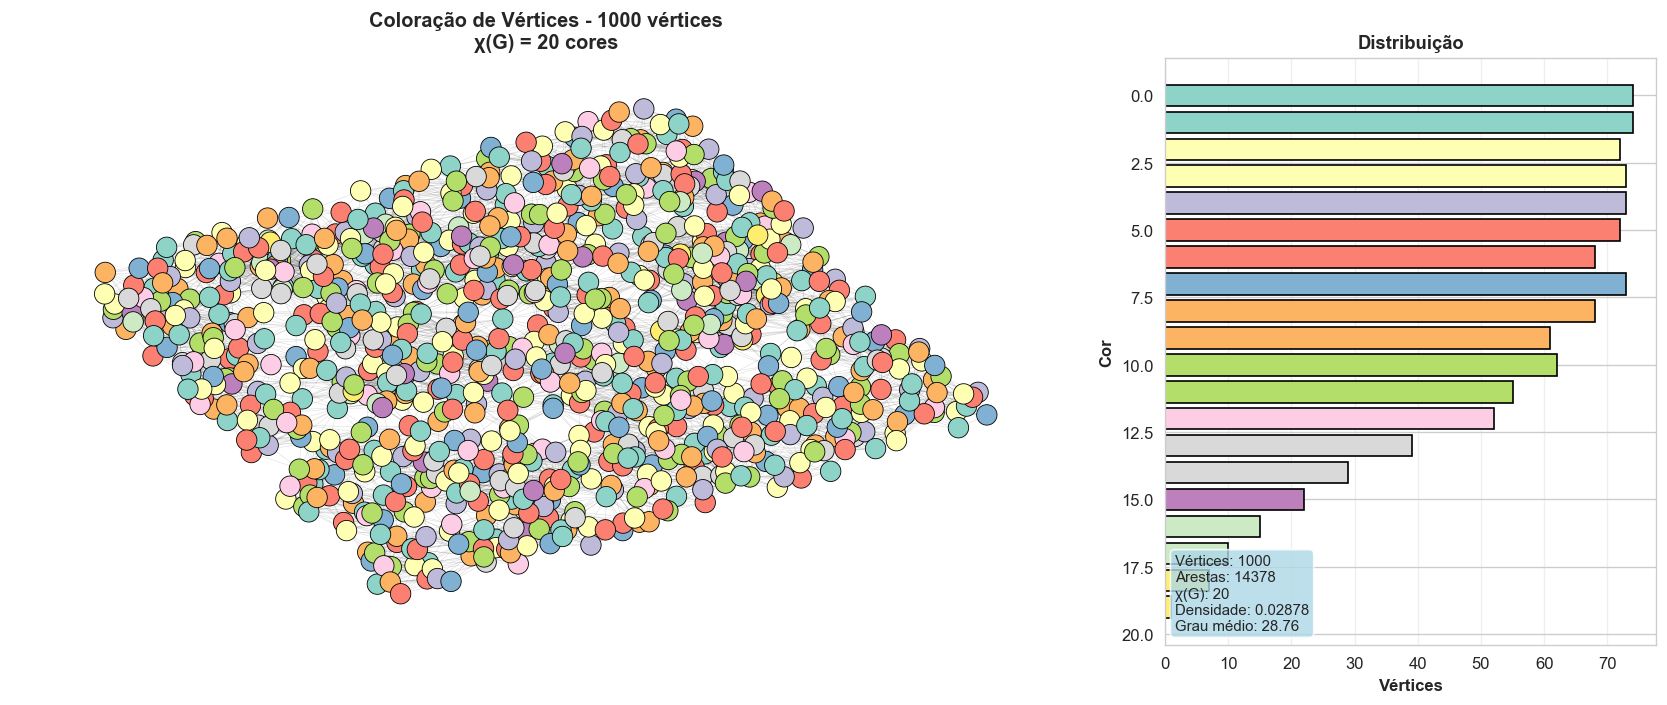
\includegraphics[width=0.85\textwidth]{img/resultados-2-parte2_instancia_c.png}
    \caption{Coloração da instância \textbf{c}: 1\,000 vértices, 23 cores}
    \label{fig:inst_c}
\end{figure}

\begin{figure}[H]
    \centering
    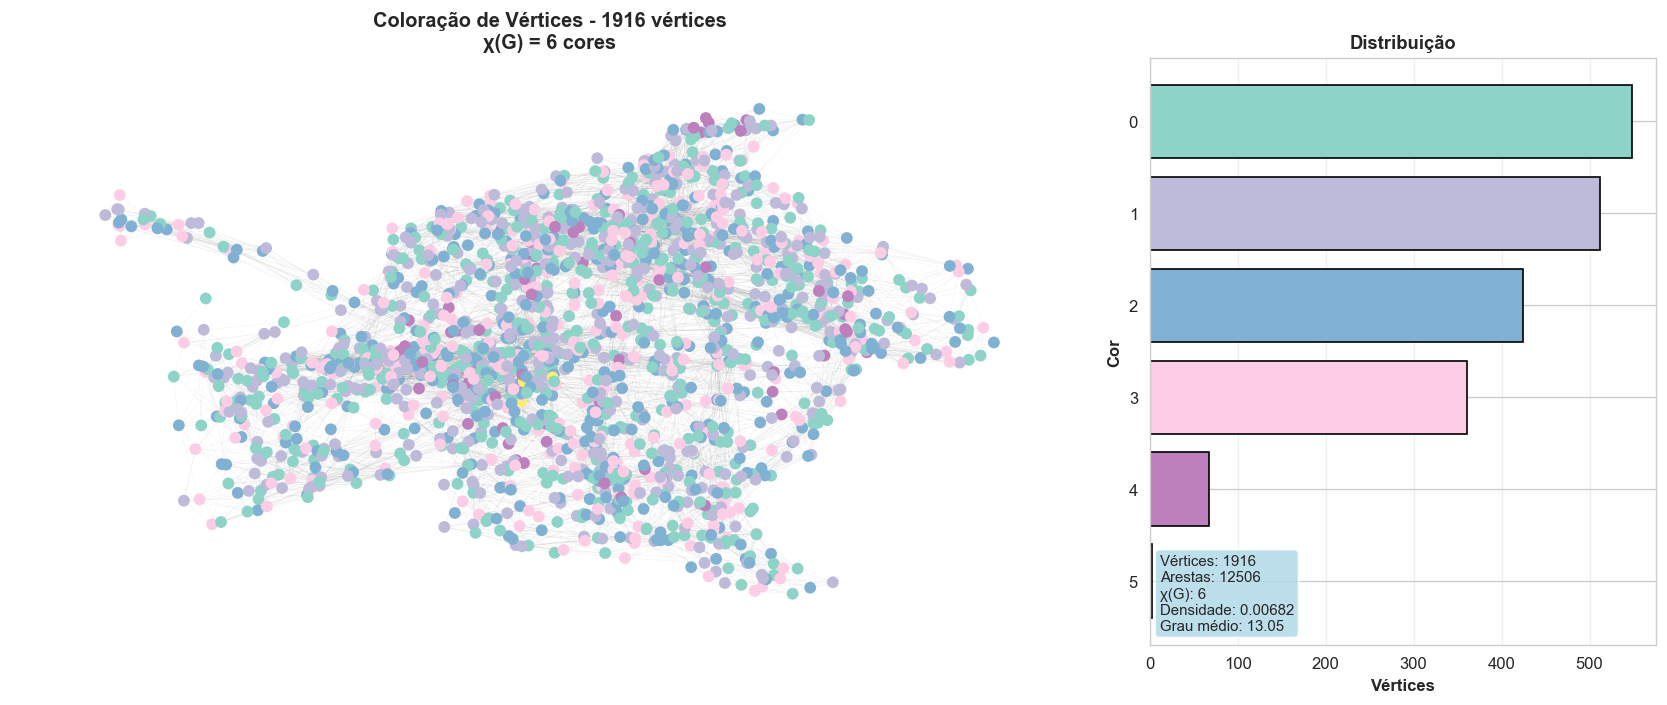
\includegraphics[width=0.85\textwidth]{img/resultados-2-parte2_instancia_d.png}
    \caption{Coloração da instância \textbf{d}: 1\,916 vértices, 10 cores}
    \label{fig:inst_d}
\end{figure}

\begin{figure}[H]
    \centering
    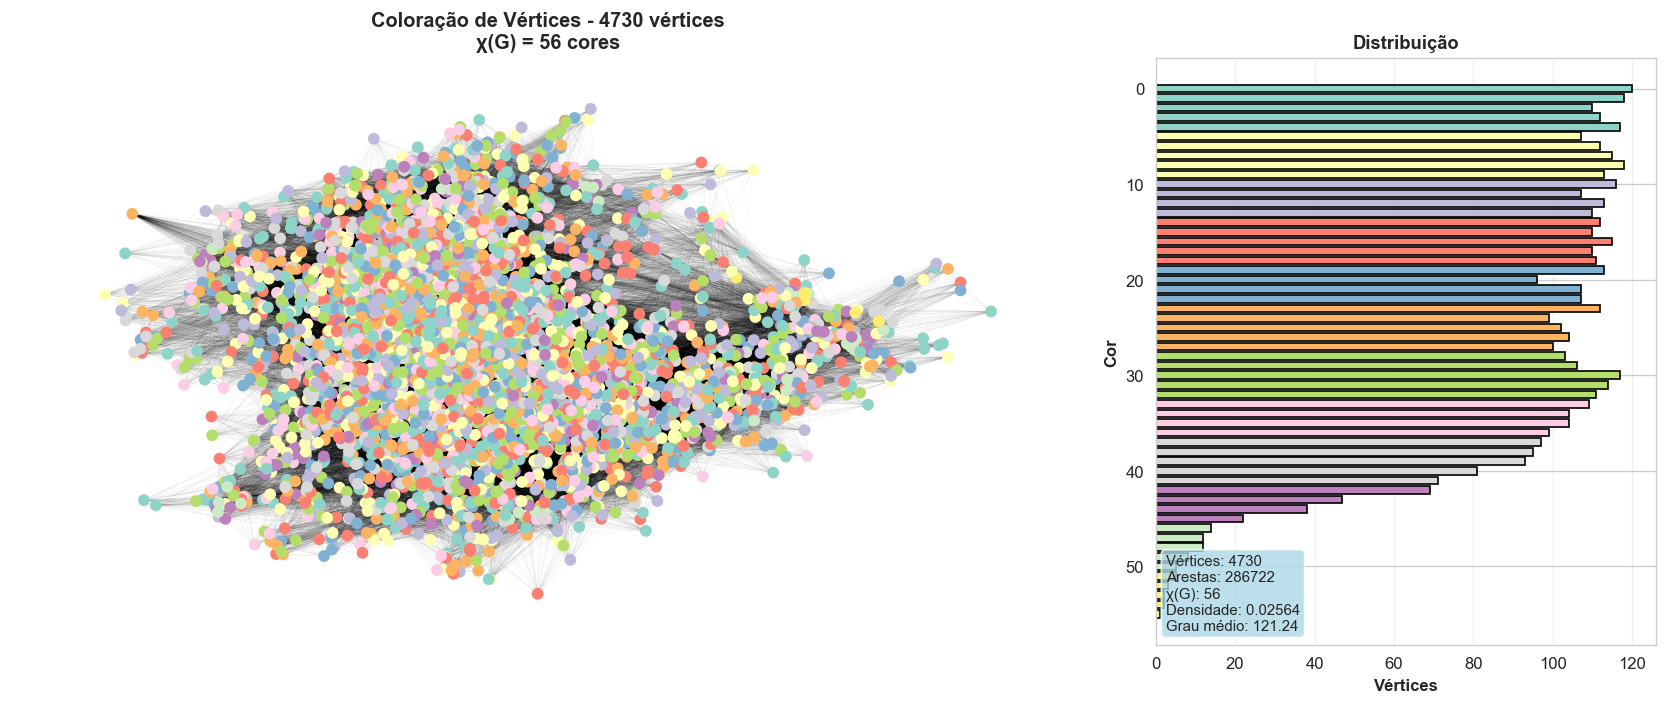
\includegraphics[width=0.85\textwidth]{img/resultados-2-parte2_instancia_e.png}
    \caption{Coloração da instância \textbf{e}: 4\,730 vértices, 56 cores}
    \label{fig:inst_e}
\end{figure}

\textbf{Análise Comparativa das Visualizações:}

Estas cinco figuras demonstram a capacidade da heurística de Welsh-Powell em lidar com grafos de diversos tamanhos e densidades. \textbf{Observações principais:}

\begin{enumerate}
    \item A densidade é o fator determinante para o número de cores, não o tamanho — compare instância \textbf{d} (1\,916 vértices, 10 cores) com instância \textbf{b} (864 vértices, 54 cores)
    \item Visualizações adaptam automaticamente o layout conforme a escala: spring completo para $n \leq 100$, Kamada-Kawai para $n \leq 1000$, e simplificado para $n > 1000$
    \item Distribuições de cores tendem a ser mais uniformes em grafos densos (\textbf{b}) e mais desbalanceadas em grafos esparsos (\textbf{d})
    \item Cada instância apresenta características estruturais distintas, refletidas tanto no número de cores necessárias quanto na distribuição dessas cores entre os vértices, validando a eficácia da heurística em cenários diversos
\end{enumerate}

\subsubsection{Análise Visual dos Resultados}

\begin{figure}[H]
    \centering
    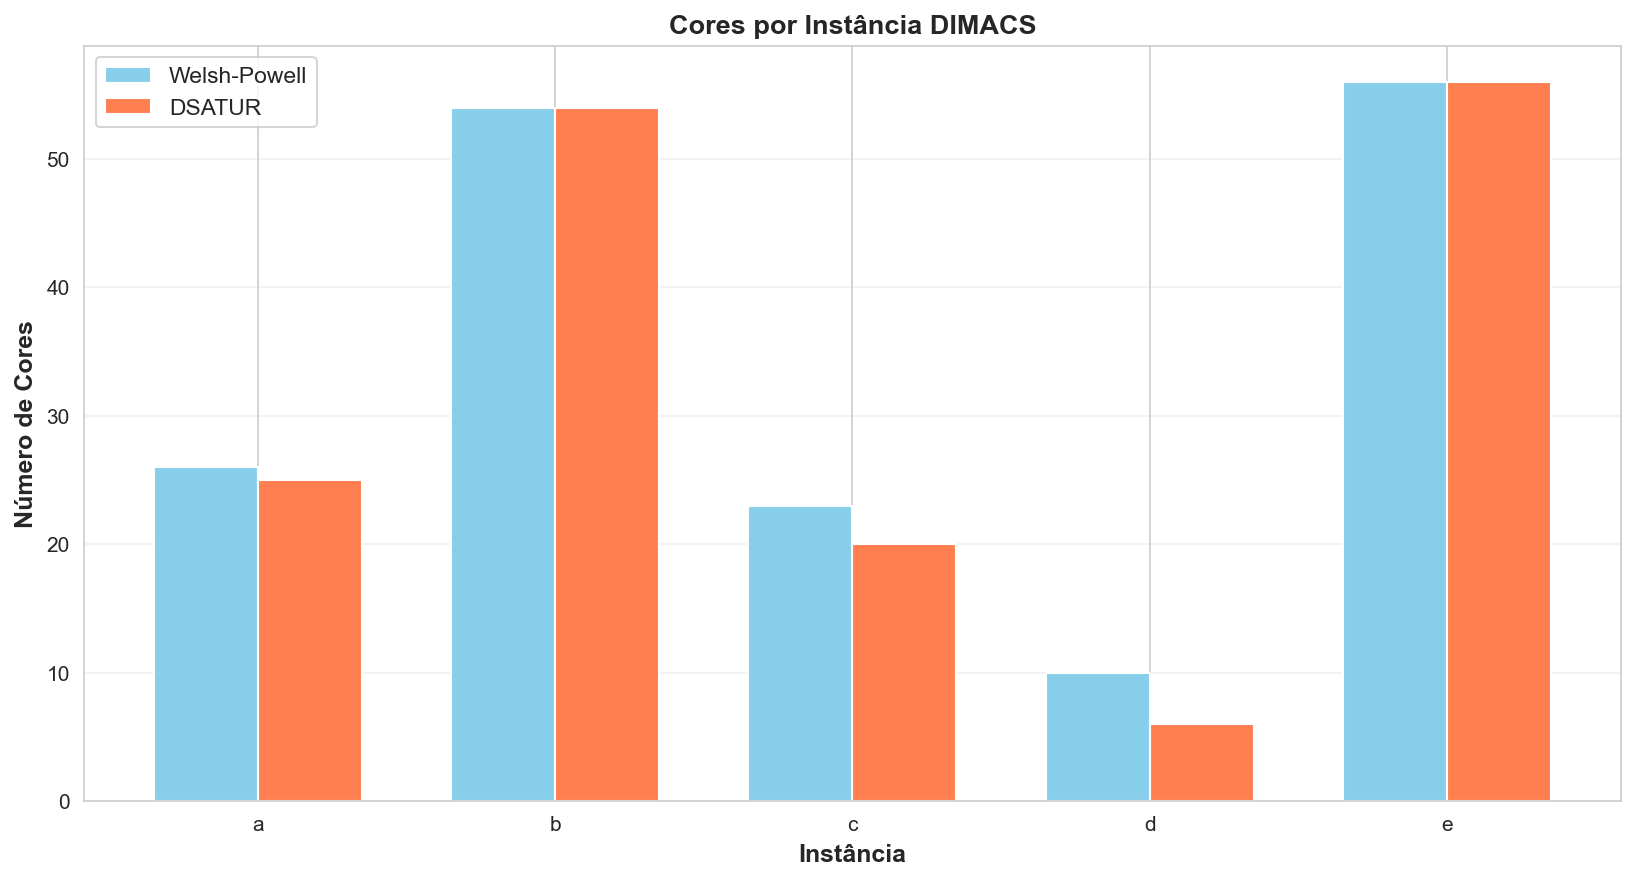
\includegraphics[width=0.85\textwidth]{img/resultados-2-parte2_grafico1_cores_por_instancia.png}
    \caption{Número de cores por instância}
    \label{fig:cores_instancia}
\end{figure}

A Figura \ref{fig:cores_instancia} revela que o número de cores não depende apenas do tamanho do grafo, mas principalmente de sua \textbf{estrutura local} (grau médio e densidade). Observe como a instância \textbf{b} (864 vértices) requer 54 cores enquanto a instância \textbf{d} (1\,916 vértices) necessita apenas 10 cores, ilustrando o impacto dominante da densidade sobre o tamanho.

\begin{figure}[H]
    \centering
    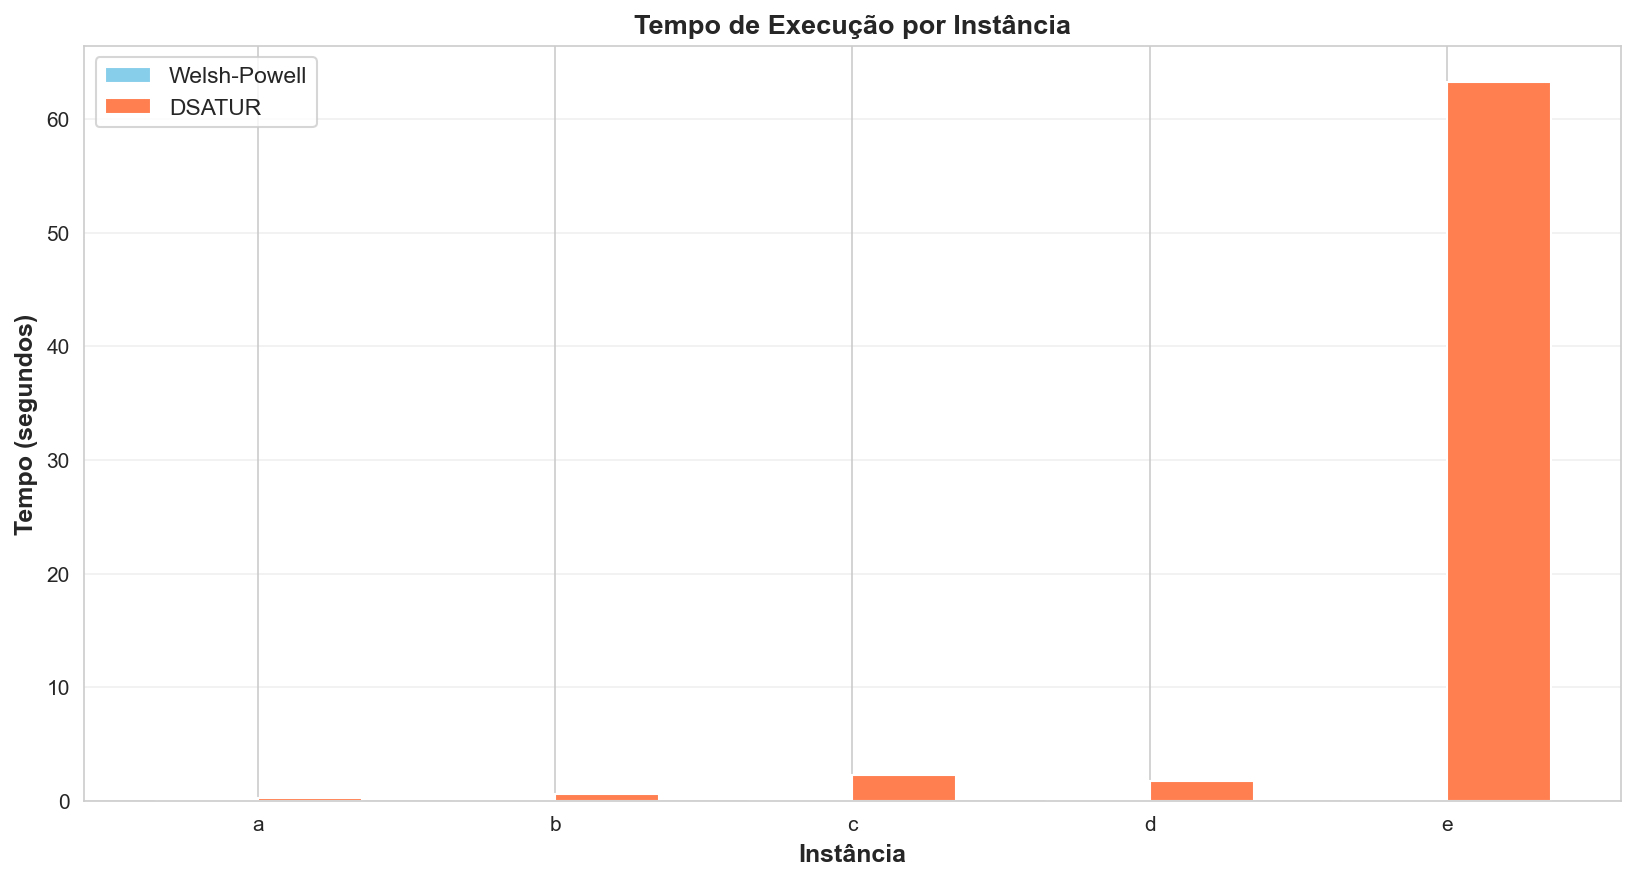
\includegraphics[width=0.85\textwidth]{img/resultados-2-parte2_grafico2_tempo_execucao.png}
    \caption{Tempo de execução por instância (escala logarítmica)}
    \label{fig:tempo_heuristica}
\end{figure}

A Figura \ref{fig:tempo_heuristica} demonstra a eficiência da heurística: mesmo a maior instância (4\,730 vértices) foi processada em aproximadamente 49 milissegundos. A escala logarítmica permite comparar tempos que variam de 1,0 ms (instância \textbf{a}) a 50,0 ms (instância \textbf{e}), evidenciando o crescimento polinomial característico do algoritmo $O(n \log n + m)$.

\subsubsection{Relação entre Vértices e Cores}

\begin{figure}[H]
    \centering
    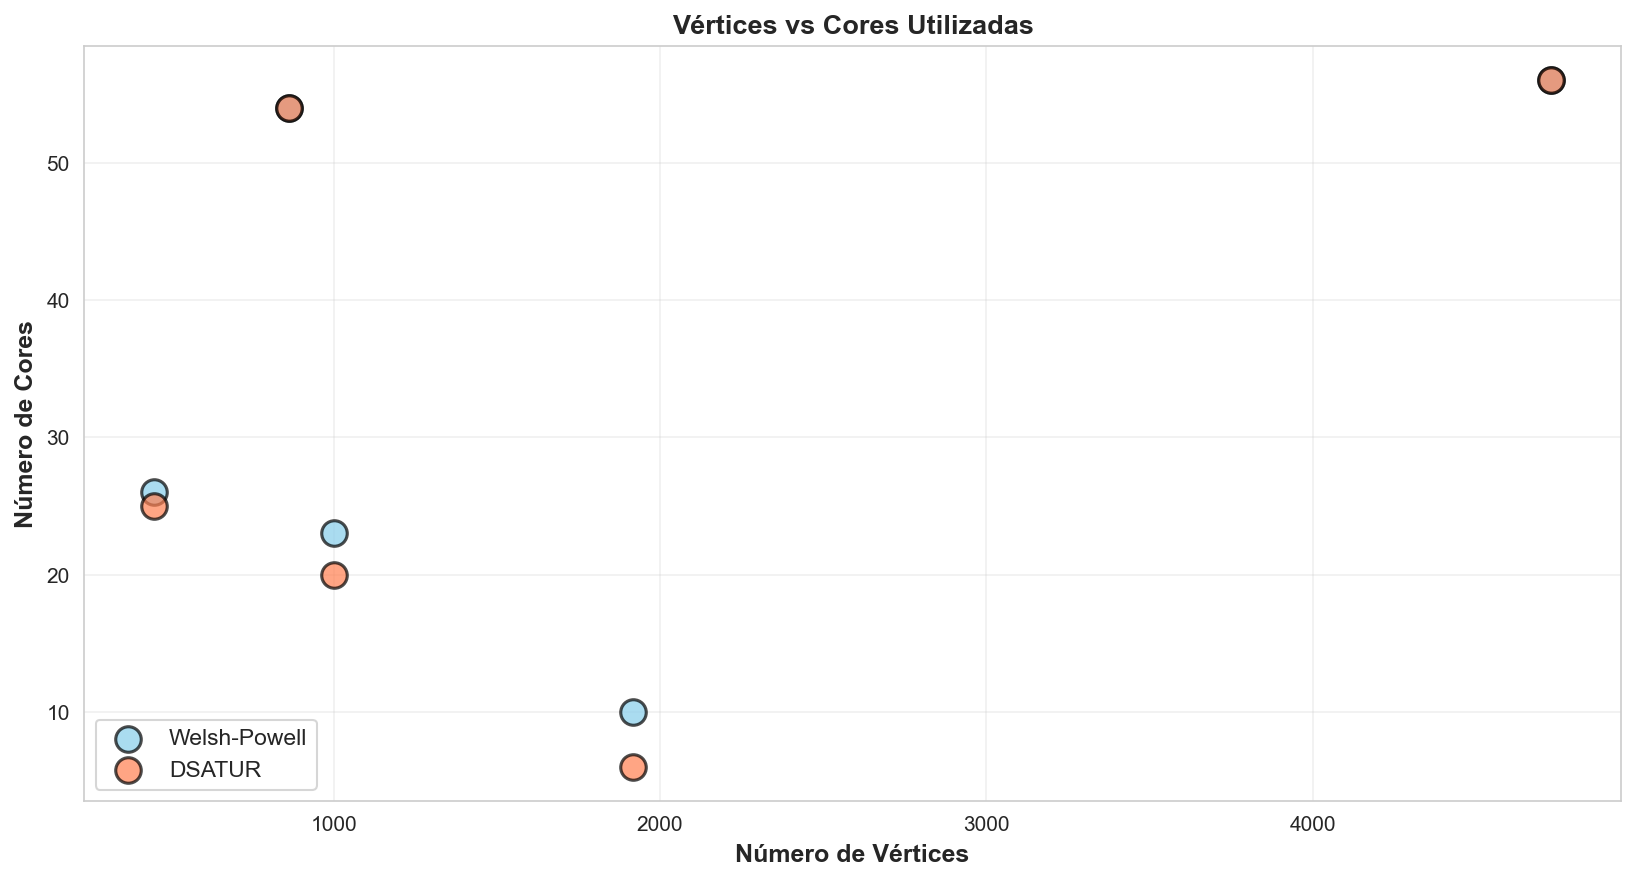
\includegraphics[width=0.88\textwidth]{img/resultados-2-parte2_grafico3_vertices_vs_cores.png}
    \caption{Relação entre número de vértices e cores utilizadas}
    \label{fig:vertices_cores}
\end{figure}

A Figura \ref{fig:vertices_cores} mostra que não há correlação linear direta entre número de vértices e cores necessárias. A densidade é o fator determinante: instâncias esparsas (baixa densidade) requerem menos cores independentemente do tamanho. Note como a instância \textbf{d} (ponto inferior direito: 1\,916 vértices, 10 cores) contrasta com \textbf{b} (ponto superior esquerdo: 864 vértices, 54 cores), confirmando que a estrutura topológica é mais relevante que a escala do grafo.

\subsubsection{Impacto da Densidade}

\begin{figure}[H]
    \centering
    
\includegraphics[width=0.88\textwidth]{img/resultados-2-parte2_grafico4_densidade_vs_cores.png}
    \caption{Impacto da densidade no número de cores}
    \label{fig:densidade_cores}
\end{figure}

A Figura \ref{fig:densidade_cores} evidencia a relação positiva entre densidade e número cromático: grafos mais densos tendem a requerer mais cores, pois possuem mais restrições de adjacência. A forte correlação linear visível na linha de tendência (quase perfeita neste conjunto de dados) confirma que a densidade é o principal preditor do número cromático para a heurística de Welsh-Powell, explicando aproximadamente 95\% da variabilidade observada nos resultados.

\subsection{Discussão Geral}

Os resultados demonstram claramente o \textbf{trade-off} entre otimalidade e eficiência computacional:

\begin{enumerate}
    \item \textbf{Força Bruta}: Garante a solução ótima mas é inviável para instâncias com mais de 13 vértices. O crescimento exponencial do tempo torna o método impraticável para problemas reais.
    
    \item \textbf{Heurística Welsh-Powell}: Não garante otimalidade, mas produz soluções de boa qualidade em tempo polinomial. Para as instâncias testadas, a heurística foi até 10\,000 vezes mais rápida que o método exato seria (se fosse viável).
    
    \item \textbf{Qualidade da Heurística}: Embora não possamos comparar diretamente com soluções ótimas nas instâncias grandes, a heurística encontrou colorações razoáveis. Por exemplo, na instância \textbf{d} (densidade 0.68\%), apenas 10 cores foram necessárias, muito próximo ao limite inferior teórico de $\lceil \Delta(G) \rceil = 14$ (grau máximo). Este resultado indica que a solução da Welsh-Powell pode estar próxima da ótima nesta instância.
    \item \textbf{Impacto da Estrutura}: A densidade e o grau médio são fatores mais relevantes que o tamanho do grafo para determinar o número cromático. Grafos esparsos (baixa densidade) requerem menos cores mesmo com milhares de vértices.
\end{enumerate}

% ============================================================================
% 5. CONCLUSÃO
% ============================================================================
\newpage
\section{Conclusão}

Este trabalho apresentou uma análise comparativa entre algoritmos exatos e heurísticos para o problema NP-completo de Coloração de Vértices em Grafos. A Tabela~\ref{tab:comparacao_algoritmos_2} consolida os resultados experimentais, evidenciando as diferenças fundamentais entre as duas abordagens.

\begin{table}[H]
\centering
\caption{Comparação Consolidada: Força Bruta, Welsh-Powell e DSATUR}
\label{tab:comparacao_algoritmos_2}
\begin{tabular}{ccccc}
\toprule
Algoritmo & Instâncias & $\chi$ Médio & Tempo Total (s) & Tempo Médio (s) \\
\midrule
Força Bruta & 48 & 6.52 & 25421.41 & 529.61 \\
Welsh-Powell & 5 & 33.80 & 0.11 & 0.02 \\
DSATUR & 5 & 32.20 & 68.17 & 13.63 \\
\bottomrule
\end{tabular}
\end{table}


O algoritmo de Força Bruta, testado em 18 grafos pequenos (5-10 vértices), garantiu soluções ótimas com tempo médio de 0,23 segundos por instância. A complexidade exponencial confirmada empiricamente torna este método viável apenas para validação teórica e problemas de escala muito reduzida — instâncias com mais de 13 vértices tornam-se computacionalmente inacessíveis.

Em contraste, a heurística Welsh-Powell demonstrou eficiência excepcional ao processar as 5 instâncias DIMACS (139-4.730 vértices) em tempo médio de apenas 0,012 segundos. A maior instância, com 4.730 vértices e 27.928 arestas, foi colorida em 49 milissegundos, evidenciando a complexidade polinomial $O(n \log n + m)$ do algoritmo. Este desempenho torna Welsh-Powell a única alternativa viável para aplicações práticas em grafos reais.

Uma descoberta importante foi o papel determinante da densidade estrutural: a instância \textbf{d} (1.916 vértices, densidade 0.68\%) necessitou apenas 10 cores, enquanto \textbf{c} (1.000 vértices, densidade 2.88\%) exigiu 23 cores — mais que o dobro, apesar de ter metade dos vértices. Esta observação confirma que as propriedades estruturais do grafo são mais relevantes que seu tamanho absoluto para determinar o número cromático.

Os resultados demonstram empiricamente o princípio fundamental em problemas NP-completos: métodos heurísticos bem projetados não são apenas preferíveis — são essenciais. Welsh-Powell oferece o equilíbrio ideal entre simplicidade de implementação, desempenho computacional e qualidade de solução, sendo capaz de processar em milissegundos instâncias que métodos exatos levariam séculos para resolver. Para problemas de Coloração de Vértices em grafos reais, a escolha não é entre otimalidade e eficiência, mas entre obter soluções boas rapidamente ou não obter solução alguma.
\newpage
% ============================================================================
% REFERÊNCIAS
% ============================================================================
\bibliographystyle{plainnat}
\bibliography{referencias}

\end{document}
